% LuaLaTeX文書; 文字コードはUTF-8
\documentclass[unicode,12pt]{beamer}% 'unicode'が必要
\usepackage{luatexja}% 日本語したい
\usepackage[ipaex]{luatexja-preset}% IPAexフォントしたい
\renewcommand{\kanjifamilydefault}{\gtdefault}% 既定をゴシック体に

\usepackage{amssymb,amsmath,ascmac}

\usepackage{multirow}
\usepackage{bm}

\graphicspath{{../fig/}}

\usepackage{tikz}
\usepackage{xparse}
\usetikzlibrary{shapes,arrows}
%% define fancy arrow. \tikzfancyarrow[<option>]{<text>}. ex: \tikzfancyarrow[fill=red!5]{hoge}
\tikzset{arrowstyle/.style n args={2}{inner ysep=0.1ex, inner xsep=0.5em, minimum height=2em, draw=#2, fill=black!20, font=\sffamily\bfseries, single arrow, single arrow head extend=0.4em, #1,}}
\NewDocumentCommand{\tikzfancyarrow}{O{fill=black!20} O{none}  m}{
\tikz[baseline=-0.5ex]\node [arrowstyle={#1}{#2}] {#3 \mathstrut};}

%目次スライド
\AtBeginSection[]{
  \frame{\tableofcontents[currentsection]}
}
%アペンディックスのページ番号除去
\newcommand{\backupbegin}{
\newcounter{framenumberappendix}
\setcounter{framenumberappendix}{\value{framenumber}}
}
\newcommand{\backupend}{
\addtocounter{framenumberappendix}{-\value{framenumber}}
\addtocounter{framenumber}{\value{framenumberappendix}} 
}

%%%%%%%%%%%  theme  %%%%%%%%%%%
\usetheme{Copenhagen}
% \usetheme{Metropolis}
% \usetheme{CambridgeUS}
% \usetheme{Berlin}

%%%%%%%%%%%  inner theme  %%%%%%%%%%%
% \useinnertheme{default}

% %%%%%%%%%%%  outer theme  %%%%%%%%%%%
\useoutertheme{default}
% \useoutertheme{infolines}

%%%%%%%%%%%  color theme  %%%%%%%%%%%
%\usecolortheme{structure}

%%%%%%%%%%%  font theme  %%%%%%%%%%%
\usefonttheme{professionalfonts}
%\usefonttheme{default}

%%%%%%%%%%%  degree of transparency  %%%%%%%%%%%
%\setbeamercovered{transparent=30}

% \setbeamertemplate{items}[default]

%%%%%%%%%%%  numbering  %%%%%%%%%%%
% \setbeamertemplate{numbered}
\setbeamertemplate{navigation symbols}{}
\setbeamertemplate{footline}[frame number]

\title{粘着剤の基礎知識と評価法}
\subtitle{~ 第一章 はじめに ~}
\author[SDL Inc. 佐々木]{佐々木 裕\thanks{hsasaki@softmatters.net}}
\institute[]{元 東亞合成株式会社\\ソフトマターデザインラボ合同会社}
\date{2024/6/24}

\begin{document}

%%%%%
% 1 P
%%%%%
\maketitle

\begin{frame} 
    \tableofcontents[]
\end{frame} 


\section{自己紹介}
\subsection{自己紹介}
\begin{frame}
	\frametitle{自己紹介}
	\begin{itemize}
		\item 略歴
			\begin{itemize}
				\item 北海道大学で合成化学系の高分子化学を専攻
				\item 東亞合成(株)に入社し2024/3まで研究・開発に従事
				\item 2024/6にソフトマターデザインラボという会社を設立
			\end{itemize}
		\item  研究・開発歴
			\begin{itemize}
				\item 合成をベースとした光硬化型材料の研究開発に従事。
				\begin{itemize}
					\item 新規材料の開発において、各種の特性評価を実施
					\item その際に、レオロジー等の評価技術の重要性を痛感。
				\end{itemize}
				\item 個別の材料開発から材料評価技術の深掘りへ軸足を。
				\item シミュレーションやレオロジー等の研究活動を継続。
			\end{itemize}
		\item その経験からのモットー
			\begin{itemize}
				\item 「化学をベースに、尤もらしく」
				\item 「物理、数学、統計の考えを利用して」
				\item 「できるだけシンプルなモデルで。」
			\end{itemize}
	\end{itemize}
\end{frame}


\subsection{モットーについて}
\begin{frame}
	\frametitle{モットーについて}
		\begin{alertblock}{これまでの経験を通して感じてきたこと}
			\begin{itemize}
				\item 「化学をベースに、尤もらしく」
				\begin{itemize}
					\item 「新規なものを作り出す技術としての\alert{化学の有用性}」
					\item \textcolor{blue}{経験則を重視して、個別の理由を考えがち。}
					\item \textcolor{blue}{化学構造式で物質を設計しようとしがち}
				\end{itemize}
				\item 「物理、数学、統計の考えを利用して」
				\begin{itemize}
					\item 「\alert{事象を客観視し、普遍性を大事}にする考え方」
					\item 雑多な化学の中に\alert{シンプルな論理性を}
				\end{itemize}
				\item 「できるだけシンプルなモデルで。」
				\begin{itemize}
					\item 数学や物理で用いられる\alert{モデル化が非常に有用}
					\item 適切なモデル化で、尤もらしいストーリーを構築
				\end{itemize}
			\end{itemize}
		\end{alertblock}
\end{frame}

\subsection{考え方のコツ}
\begin{frame}
	\frametitle{考え方のコツ}
		\begin{block}{感じてきたことをまとめ直すと、}
			\begin{itemize}
				\item 化学構造式と実際の物性の関係は非常に複雑。
				\begin{itemize}
					\item ややこしいものを、全部理解しようとしても無理。
					\item かと言って、単純化しすぎても役に立たない。
				\end{itemize}
				\item 「なぜそうなっているんだろう?」と考えてみる。
				\begin{itemize}
					\item 自分の言葉で理由を考えて、
					\item 人に説明できるように話の流れを作る。
					\item 流れの各ステップはできるだけ単純に。
				\end{itemize}
				\item できるだけシンプルな実験を
				\begin{itemize}
					\item 同時に仮定を複数設定しないこと。
					\item 実験前によく考えて計画を建てる。
					\item 一つずつ検証していく。
				\end{itemize}
			\end{itemize}
		\end{block}
\end{frame}

\section{本講座の進め方}
\subsection{最近の風潮}
\begin{frame}
    \frametitle{最近の風潮}
            \begin{block}{直ぐに結果を求めたがる}
                \begin{itemize}
                    \item 実事象はあまりに複雑で因果関係がわかりにくいのに、すぐに結果を求める。
                    \begin{itemize}
                        \item 具体的な対策、方法論を望む
                        \item 考え方の提示では満足しない
                    \end{itemize}
                    \item シミュレーションに対しても考え方の指針ではなく、\\答えを求める。
                    \begin{itemize}
                        \item 概念的なものをあまり重視しない。
                        \item そのようなアプローチは、汎用性を生み出さない。
                    \end{itemize}
                \end{itemize}

                    \centering
                        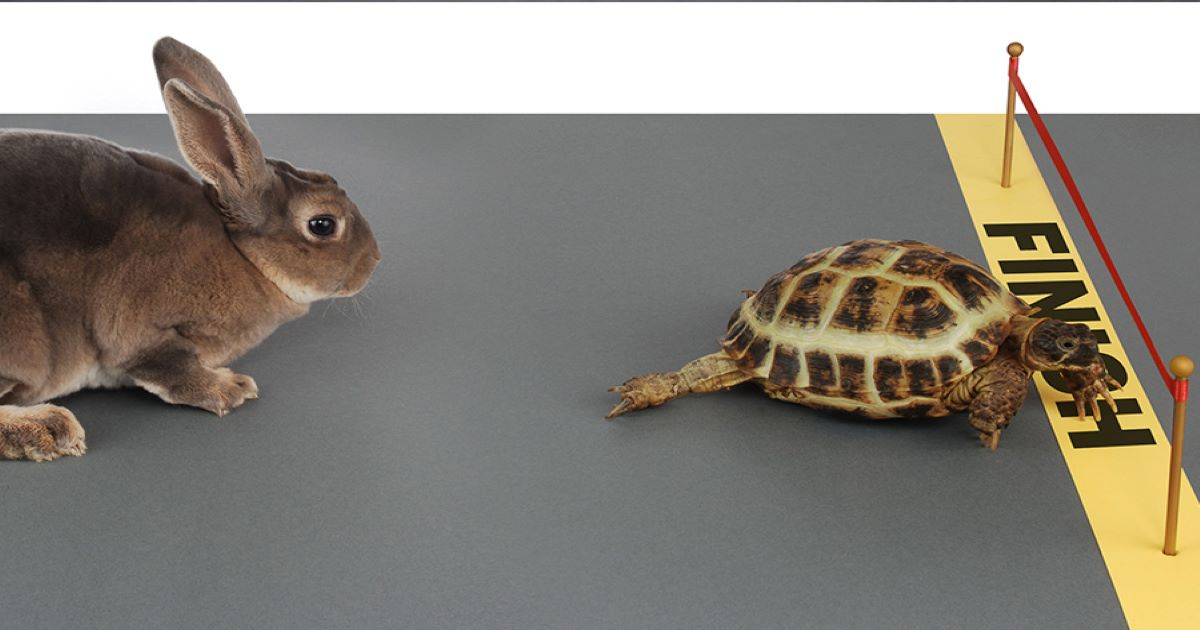
\includegraphics[width=.4\textwidth]{usagi_kame.jpg}
                
            \end{block}
\end{frame}

\subsection{理解へのアプローチ}
\begin{frame}
	\frametitle{理解へのアプローチ}
	\vspace{-2mm}
	\begin{block}{ざっくりと捕まえよう。}
		\begin{itemize}
			\item 個々の要素技術の基本を、イメージとして捉えて、
			\item 全体像をざっくりと捕まえれば、理解は一気に容易に。
		\end{itemize}
	\end{block}
	
	\pause
	\vspace{-2mm}
	\begin{alertblock}{粘着技術を簡単に言えば、}
		\begin{itemize}
			\item 粘着シートが短時間で貼り付き、
			\item その状態をそれなりの強さで維持して、
			\item 必要に応じて簡単に剥離できる。
		\end{itemize}
	\end{alertblock}

	\pause
	\vspace{-2mm}
	\begin{exampleblock}{タッキファイヤーの働きは?}
		\begin{itemize}
			\item タッキファイヤーとはどんなもので、
			\item どんな働きをしているのだろうか?
			\item なぜ、そんなふうな機能を有しているのだろうか?
		\end{itemize}
	\end{exampleblock}

\end{frame}


\subsection{見える化のすすめ}
\begin{frame}
	\frametitle{自分の中への落とし込み}
		\begin{block}{「何のためにやりたいのか?」を明確に}
			\begin{itemize}
				\item 目的がわからないと、ゴールが見えません。
				\item 仕事であれば、上司とよく相談しましょう。
				\item 自己啓発であれば、自分の本心をよく見極めましょう。
			\end{itemize}
		\end{block}
		\pause
		\begin{block}{「何をやりたいのか?」を常に意識}
			\begin{itemize}
				\item 因果関係をはっきりとつけましょう。
				\begin{itemize}
					\item 因 $\Leftarrow$ 原因
					\item 果 $\Leftarrow$ 結果
				\end{itemize}
				\item 図として捉えてみましょう。
				\begin{itemize}
					\item 複雑な実事象をできるだけ単純化して、
					\item 一目で理解できるようにしましょう。
				\end{itemize}
			\end{itemize}
		\end{block}
\end{frame}

\begin{frame}
	\frametitle{色々なモデル化}
	「さまざまな条件のもとで、幅広い検討対象に対してでも当てはめることのできるような汎用的なモデル」を考えることが役にたったと実感。
	\begin{exampleblock}{モデル化のすすめ}
		\begin{columns}[c, onlytextwidth]
			\column{.68\linewidth}
			\begin{itemize}
				\item 適度な深さで尤もらしく
					\begin{itemize}
						\item 簡単すぎるものは例外が多い。
						\item 複雑化しすぎても過適応
							\begin{itemize}
								% \item n個のデータを、n次の関数でフィット
								\item 個々の現象にだけ適応可能
								\item モデル化する意味がない
							\end{itemize}
					\end{itemize}
				\item 欲しいもの
					\begin{itemize}
						\item 汎用的に使えるモデル
						\item 尤もらしく、実験事実を説明可能
					\end{itemize}
			\end{itemize}
			\column{.3\linewidth}
					\centering
						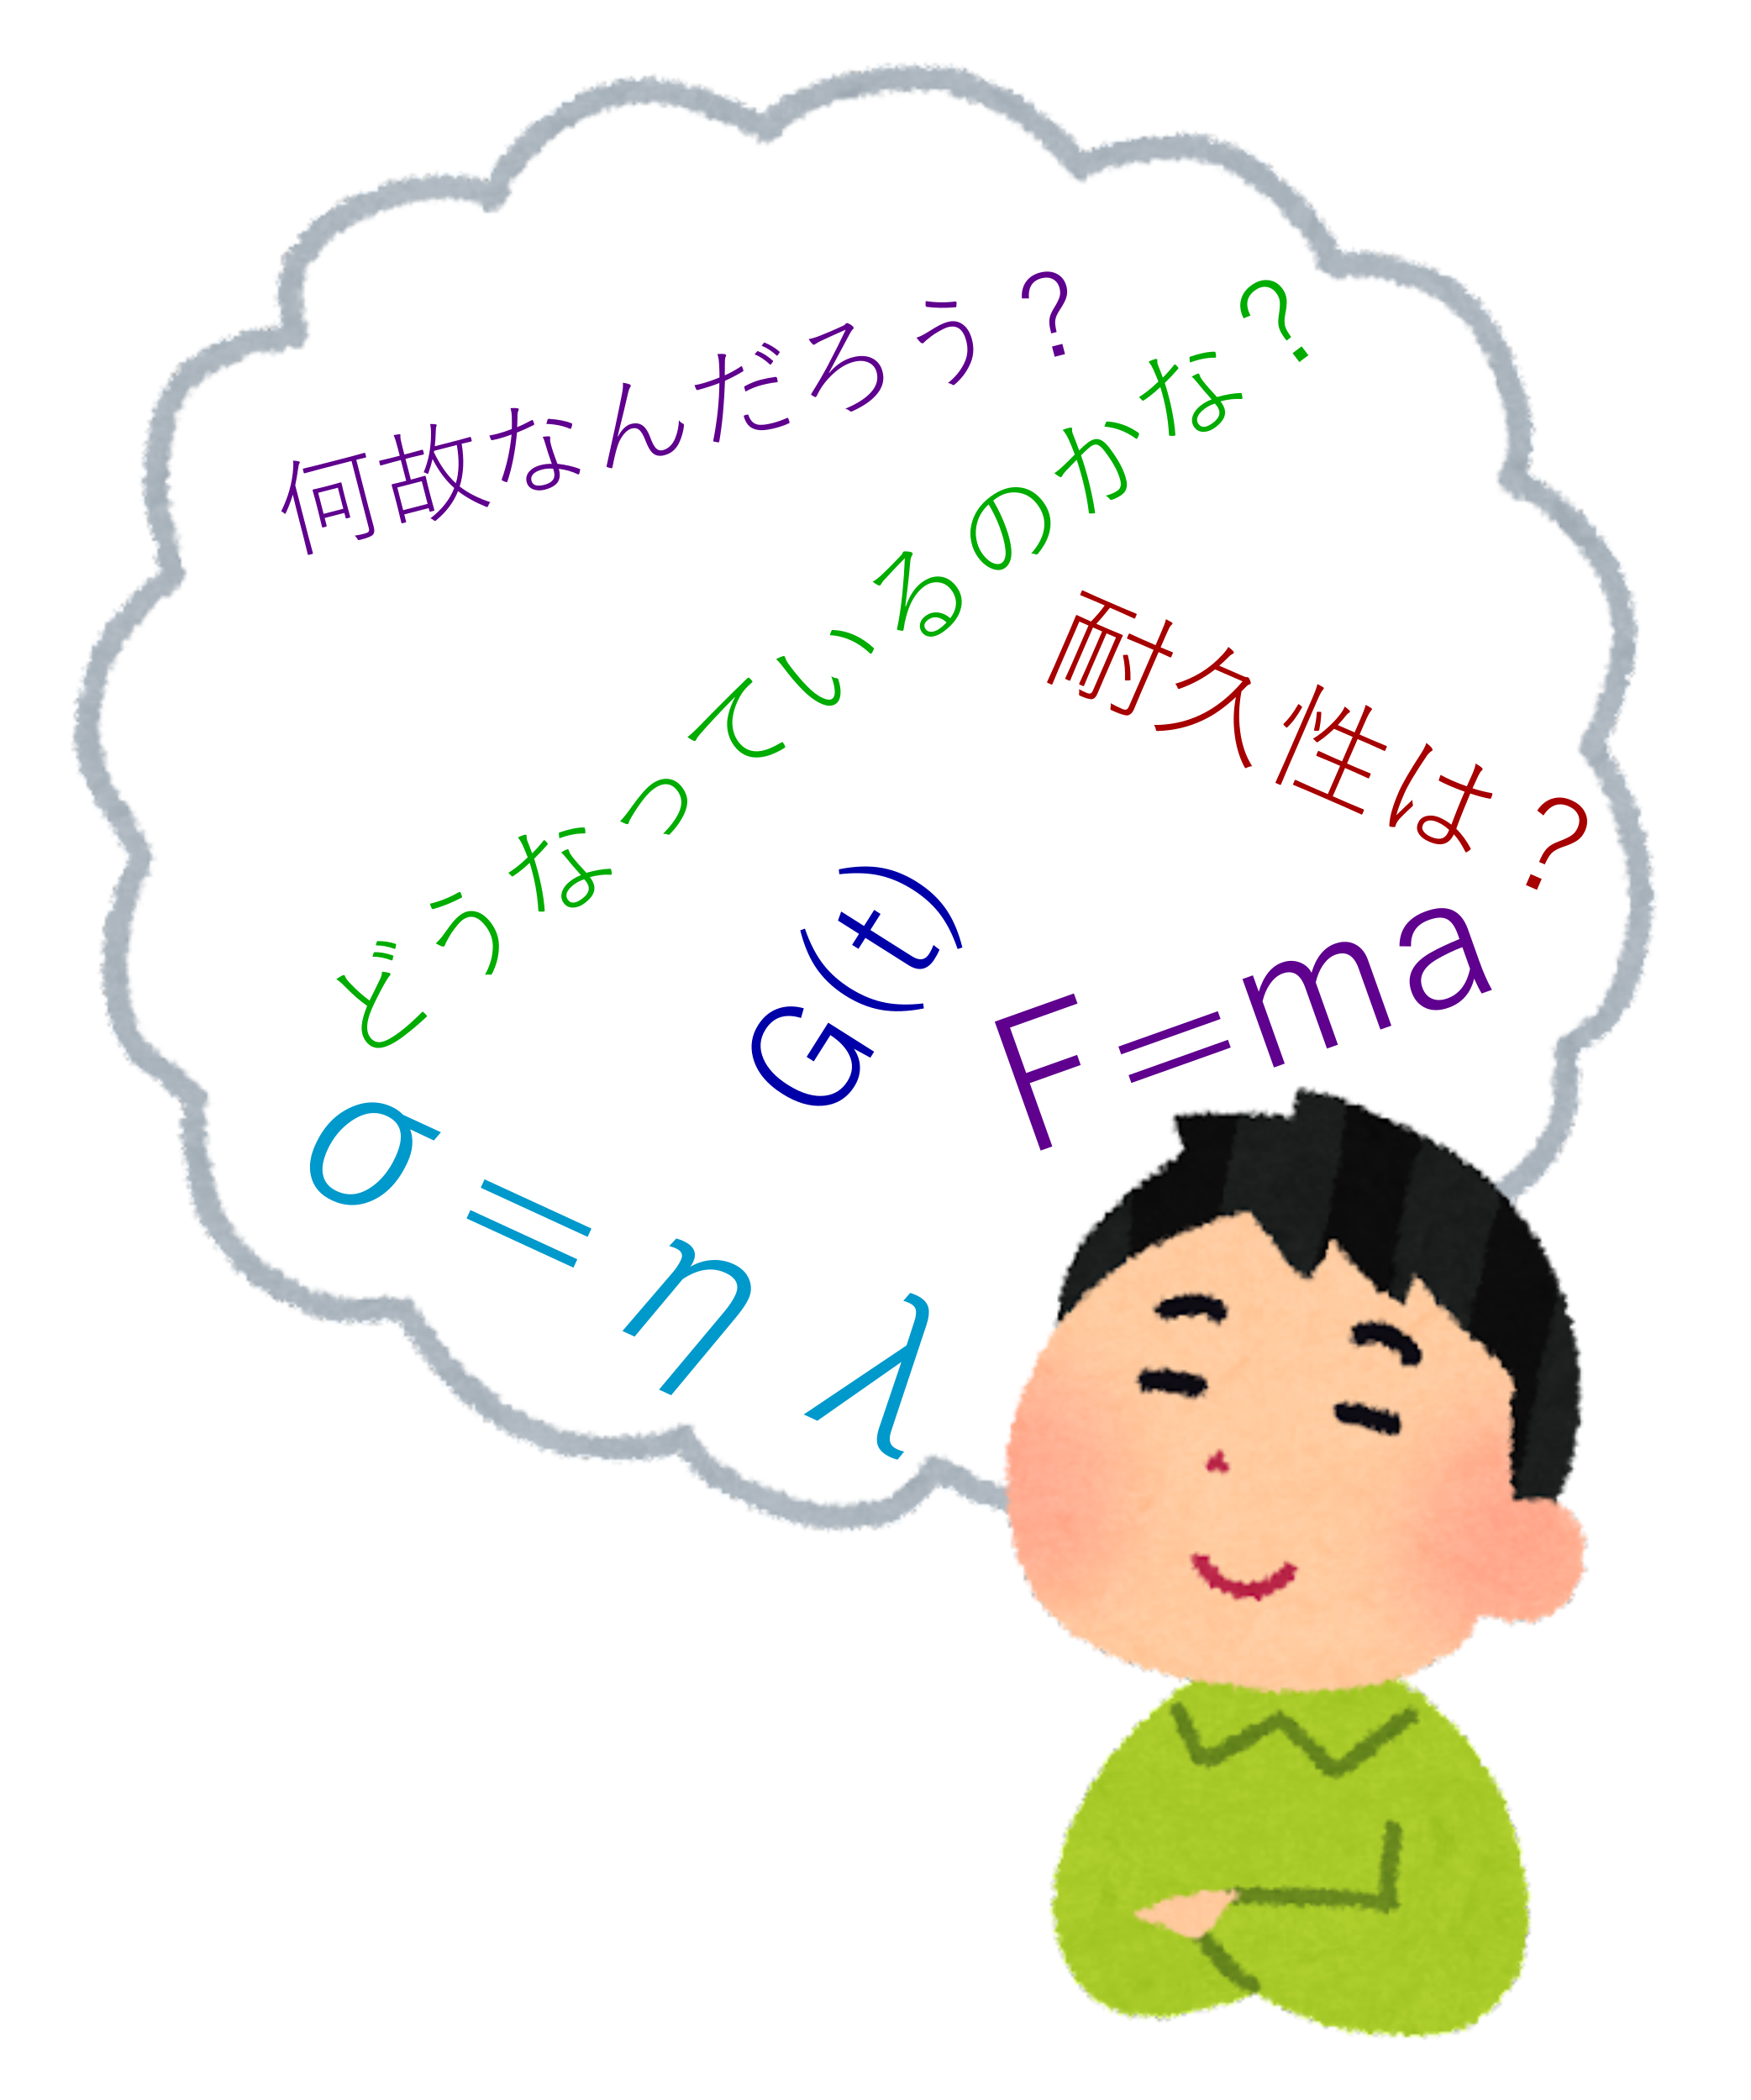
\includegraphics[width=\textwidth]{souzou.png}
		\end{columns}
	\end{exampleblock}
\end{frame}

% \subsection{目指すもの}

\begin{frame}
	\frametitle{おすすめのやり方}
	
	\begin{center}
		{\Huge \textbf{「急がば回れ」}}
	\end{center}
	
	\vspace{5mm}
	\begin{alertblock}<2->{ざっくり全体像をイメージ}
		\begin{columns}[c, onlytextwidth]
			\column{.6\linewidth}
			\begin{itemize}
				\item 慌てて結果を出そうとしない。
				\begin{itemize}
					\item 心を落ち着けて、
					\item やるべきことを、
					\item 明確にイメージする。
				\end{itemize}
				\item 全体像をザックリと捕まえる。
				\item 理解は一気に容易になり、
				\item ゴールへの道も見えてくる。
			\end{itemize}
			\column{.35\linewidth}
					\centering
						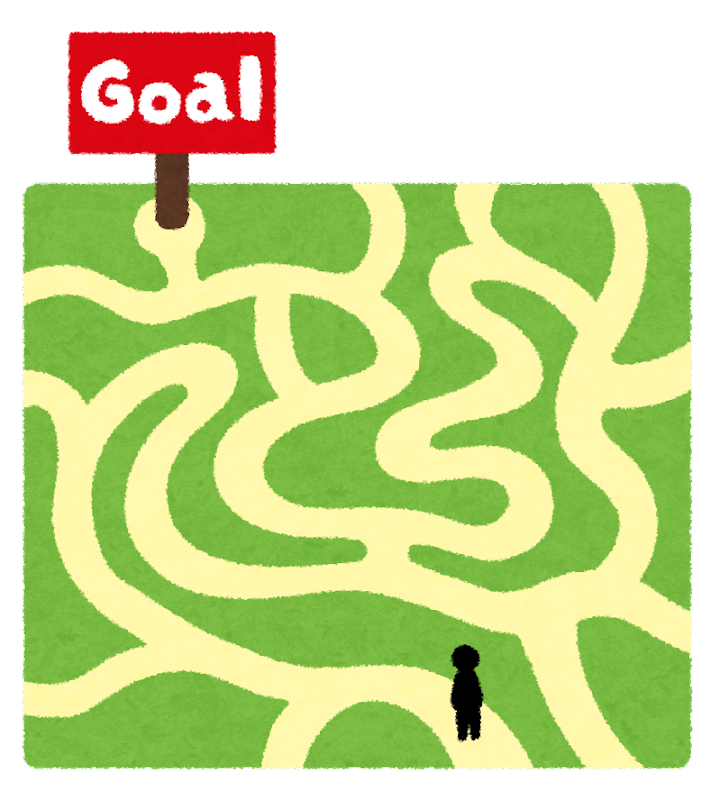
\includegraphics[width=\textwidth]{goal.png}
		\end{columns}
	\end{alertblock}
\end{frame}

\begin{frame}
	\frametitle{イメージを大事に}
		実際の研究開発に役に立つように粘着関連技術を理解していただくために、以下のような点に気を付けて、説明していきたいと考えています。
		\begin{block}{ポイント}
			\begin{itemize}	
				\item イメージしやすい、直感的な理解を目指す。
					\begin{itemize}
						\item 全体を俯瞰した概念的な説明を。
						\item 多様な切り口からの説明を。
					\end{itemize}
				\item 大事なことは何度か繰り返す。
					\begin{itemize}
						\item 一度ではわかりにくいかも。
						\item 似たような内容を、ちょっと違う言葉で。
					\end{itemize}
				\item ゆっくり議論
					\begin{itemize}
						\item わかりにくいことは遠慮なく質問を。
						\item やりたいことを伝えてください。
					\end{itemize}
			\end{itemize}
		\end{block}
\end{frame}

\begin{frame}
    \frametitle{最近の風潮}
            \begin{block}{直ぐに結果を求めたがる}
                \begin{itemize}
                    \item 実事象はあまりに複雑で因果関係がわかりにくいのに、すぐに結果を求める。
                    \begin{itemize}
                        \item 具体的な対策、方法論を望む
                        \item 考え方の提示では満足しない
                    \end{itemize}
                    \item シミュレーションに対しても考え方の指針ではなく、\\答えを求める。
                    \begin{itemize}
                        \item 概念的なものをあまり重視しない。
                        \item そのようなアプローチは、汎用性を生み出さない。
                    \end{itemize}
                \end{itemize}

                    \centering
                        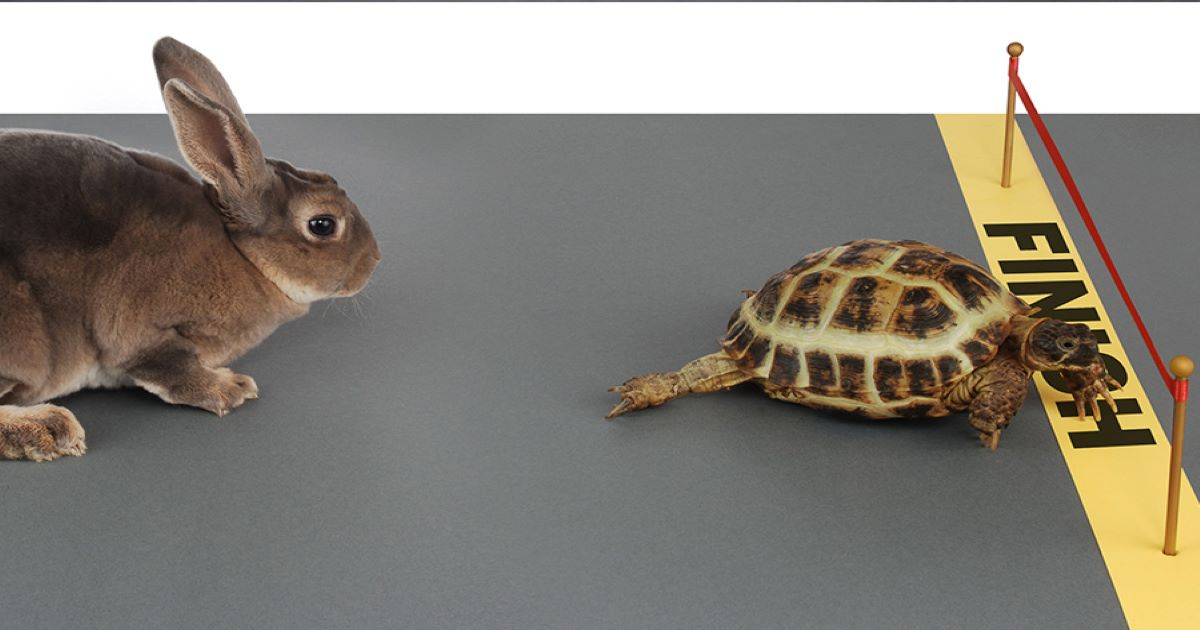
\includegraphics[width=.4\textwidth]{usagi_kame.jpg}
                
            \end{block}
\end{frame}

\end{document}